\documentclass[11pt,a4paper]{article}
\usepackage[margin=2.5cm]{geometry}
\usepackage[T1]{fontenc}
\usepackage{lmodern}
\usepackage{amsmath,amssymb,booktabs,graphicx,enumitem,xcolor,caption}
\usepackage[round,authoryear]{natbib}
\usepackage[colorlinks=true,linkcolor=black,citecolor=black,urlcolor=blue]{hyperref}
\setlist{itemsep=2pt,topsep=4pt}
\captionsetup{font=small,labelfont=bf}
\newcommand{\musd}{USD~million}

\title{Build for today, adapt tomorrow:\\ technology choice under demand uncertainty in least-cost electrification planning\\[4pt]
\large Evidence from 128,000 off-grid settlements in Madagascar}
\author{Felix C.\,L. Mergenhagen\thanks{DIW Berlin and Technische Universit\"at Berlin. Draft prepared with the
assistance of an AI model; code and results are in the accompanying repository
(\texttt{national/}, \texttt{onsset\_madagascar/}, \texttt{swarmplan/}, \texttt{case\_study/}).}}
\date{Working draft v0.1, 16 November 2026}

\begin{document}
\maketitle
\vspace{-1.2em}
\begin{center}
\fbox{\parbox{0.92\textwidth}{\small\textbf{Status.} Preliminary. The OnSSET inputs are of 2019 vintage, part of the
model specification is assumed, and the swarm-grid cost parameters are not yet based on field data
(Section~\ref{sec:limits}). Numbers will change. Not for citation.}}
\end{center}

\begin{abstract}
\noindent Geospatial least-cost models assign one technology to each settlement for an assumed level of demand.
Using OnSSET for Madagascar, we show that this assignment is unstable: between a low and a high rural demand
target, 11.3 million people (32\,\% of the 2030 population) move from stand-alone solar to mini-grids, and
investment rises from USD 3.8 to 12.2 billion. We then treat demand as uncertain in a two-stage decision model for
128,065 off-grid settlements with 17 million people. Three results follow. First, building for the high target from
the outset costs 2.4 times as much as building for current demand and adapting if demand rises with probability
25\,\%, and still a third more if the rise is certain. Second, this simple adaptive rule is within 0.5\,\% of the
stochastic optimum for probabilities up to one half, and perfect foresight is worth less than 1\,\%. Third, an
intermediate swarm-grid option lowers expected cost by 1 to 2\,\% in our central case and by up to 11\,\% if
distributed generation carries no cost premium; hardware that survives an upgrade is worth more, 2 to 3\,\%.
The value lies in modularity, not in forecasting.

\medskip\noindent\textbf{Keywords:} electricity access, demand uncertainty, staged investment, swarm electrification,
mini-grids, geospatial planning, Madagascar. \quad \textbf{JEL:} O13, Q41, Q48, D81, L94.
\end{abstract}

\section{Introduction}
National electrification plans are increasingly built with geospatial least-cost models such as OnSSET
\citep{mentis2017} and the Reference Electrification Model \citep{rem2018}. For every settlement these tools pick the
cheapest of grid extension, a mini-grid or stand-alone systems. The choice depends on how much electricity people
are assumed to use, and that is the least known input. Newly connected rural households often consume very little
\citep{lee2019}, and plans that are least-cost on paper frequently cannot be financed or implemented
\citep{diazpastor2026}.

Swarm electrification has been proposed as a way around the dilemma: start with small solar systems, interconnect
them step by step, and upgrade when demand justifies it \citep{groh2014,kirchhoff2019,sheridan2023}. The claimed
advantage is that investment follows demand instead of running ahead of it. Existing swarm models, however, study
a single community in a single design year \citep{hoffmann2019,bertram2024,dumitrescu2022,ouanes2026}, while multi-year stochastic planning has been
developed for mini-grids alone \citep{fioriti2021}. Whether a modular middle option matters at the scale of a
national plan, and how much, has not been quantified.

This paper makes three contributions. (i) It measures how unstable a least-cost plan is with respect to the demand
assumption, settlement by settlement. (ii) It embeds OnSSET's own cost estimates in a two-stage decision model with
uncertain demand and compares four planning rules. (iii) It adds a swarm-grid option whose cost is derived from
OnSSET's mini-grid cost through additional model runs, and maps the conditions under which the option has value.

\section{Data and baseline}
We use the Global Electrification Platform inputs for Madagascar: 155,275 settlements, 27.7 million people in 2020
and 35.6 million in 2030, of whom 31\,\% are electrified at the start. OnSSET is run for 2020--2030 under the two
demand targets of the platform's Madagascar model \citep{gep2019}: \emph{low} (urban Tier~3, rural Tier~1 of the
multi-tier framework) and \emph{high} (urban Tier~4, rural Tier~3). Table~\ref{tab:base} and
Figure~\ref{fig:map} summarise the outcome.

\begin{table}[!ht]\centering\small
\caption{Least-cost plans for 2030 under two demand targets (million people).}\label{tab:base}
\begin{tabular}{lrr}\toprule
 & Low demand & High demand\\\midrule
Grid (existing and new) & 14.7 & 16.3\\
Mini-grids & 6.3 & 17.2\\
Stand-alone solar & 14.6 & 2.0\\
Investment 2020--2030 (USD billion) & 3.8 & 12.2\\\midrule
\multicolumn{3}{l}{People who change technology class between the two plans: 39\,\%}\\
\multicolumn{3}{l}{\quad of which stand-alone solar $\rightarrow$ mini-grid: 11.25 million (32\,\%)}\\\bottomrule
\end{tabular}
\end{table}

\begin{figure}[!ht]\centering
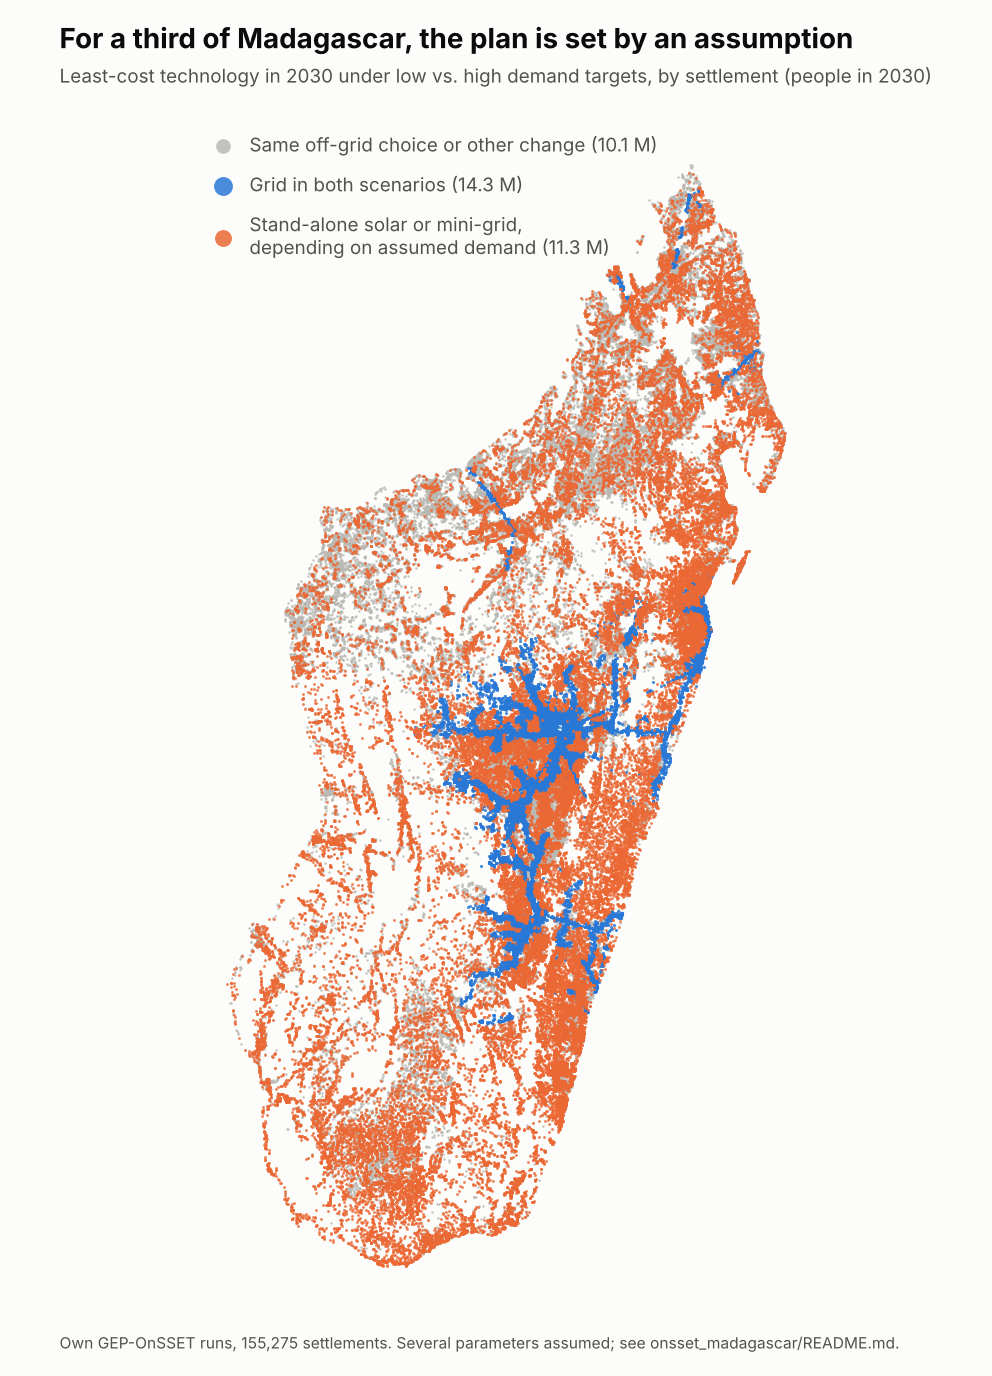
\includegraphics[width=0.56\textwidth]{fig_madagascar_switch.png}
\caption{Settlements by how their least-cost technology responds to the demand target.}\label{fig:map}
\end{figure}

For a third of the population the plan is therefore determined by an assumption. The investment requirement triples.
For comparison, the national integrated energy access plan puts the cost of universal access by 2030 at about
USD 7 billion, excluding new grid generation and transmission, and assigns roughly half of its 9 million new
connections to stand-alone solar and a fifth to mini-grids \citep{seforall2024}.

\section{Model}\label{sec:model}
\subsection{Domain and costs}
The analysis covers the 128,065 settlements that are unelectrified in 2020 and are not reached by the grid in either
baseline plan (17.0 million people in 2025). For technology $k$ and demand level $d\in\{L,H\}$, OnSSET's first-step
levelised cost and the settlement's annual energy demand give the annual cost
\begin{equation}
A_{kd}=\mathrm{LCOE}_{kd}\cdot E_d \qquad\text{(USD per year)} .
\end{equation}
Technologies are stand-alone solar (SA), a conventional mini-grid (MG; the cheapest of PV-hybrid, hydro and
wind-hybrid) and, in the extended menu, a swarm grid (SW).

\subsection{Two-stage decision}
Stage~1 covers years 1--5, stage~2 years 6--15; the discount rate is 8\,\%, which gives stage weights
$w_1=0.466$ and $w_2=0.534$. Demand is low in stage~1. In stage~2 it stays low with probability $1-p$ or rises to
the high level with probability $p$. A first-stage action is a technology and a size, $a=(k,s)$.

\emph{Sized for low demand}, $a=(k,L)$. The system costs $A_{kL}$ while demand is low. If demand rises it can be
expanded in place or replaced by technology $j$, in which case the share $(1-\chi_{kj})$ of its capital is stranded:
\begin{equation}
C^{H}_{2}(k,L)=\min\Big\{A_{kH},\ \min_{j\neq k}\big[A_{jH}+(1-\chi_{kj})\,\sigma_k A_{kL}\big]\Big\},
\end{equation}
where $\sigma_k$ is the capital share of levelised cost and $\chi_{kj}\in[0,1]$ the share of $k$'s hardware that
remains useful under $j$.

\emph{Sized for high demand}, $a=(k,H)$. The system costs $A_{kH}$ once demand is high. While demand is low it costs
its capital share plus the running cost of the energy actually used,
$\bar A_{kH}=\sigma_kA_{kH}+(1-\sigma_k)A_{kH}\,E_L/E_H$.

Expected cost is
\begin{equation}
EC(a)=w_1C_1(a)+w_2\big[(1-p)\,C_2^{L}(a)+p\,C_2^{H}(a)\big].
\end{equation}
We compare four rules: \emph{build for the high target} (the technology that is cheapest at high demand, sized for
it from day one); the \emph{adaptive rule} (the technology that is cheapest at current demand, sized for it,
re-optimised if demand rises); the \emph{stochastic optimum} ($\min_a EC(a)$); and \emph{perfect information}
(the best action in each demand path). Central values are $\sigma_{SA}=0.85$, $\sigma_{MG}=\sigma_{SW}=0.75$,
$\chi_{SA,MG}=0$ and $\chi_{SA,SW}=\chi_{SW,MG}=1$.

\subsection{A swarm-grid option on OnSSET's cost basis}
OnSSET's mini-grid cost is linear in the fixed cost per system $F$ (USD 10,000) and in the unit cost of low-voltage
lines $c$ (USD 4,250 per km). Two additional runs per demand level, one with $F=2{,}500$ and one with $F=2{,}500$
and $c=2{,}000$, identify for every settlement the decomposition
\begin{equation}
A^{MG\text{-}PV}_{d}=G_d+\ell_d\,c+\phi_d\,F ,
\end{equation}
with $G_d$ the cost of generation, storage and connections. A swarm grid is modelled as
\begin{equation}
A^{SW}_{d}=(1+\pi)\,G_d+\ell_d\,c_{SW}+\phi_d\,F_{SW}:
\end{equation}
a smaller fixed cost and cheaper lines, but generation that is more expensive by the premium $\pi$ because it is
built in small distributed units. The central case is $\pi=0.30$, $F_{SW}=2{,}500$, $c_{SW}=2{,}000$; all three are
assumptions and are varied below.

\section{Results}
\subsection{Cost structure}
\begin{table}[!ht]\centering\small
\caption{Cost by technology and demand level, off-grid domain.}\label{tab:cost}
\begin{tabular}{lrrrr}\toprule
 & \multicolumn{2}{c}{USD per person and year} & \multicolumn{2}{c}{Cheapest for (million people)}\\
 & Low & High & Low & High\\\midrule
Stand-alone solar & 24.1 & 139.7 & 11.7 & 1.5\\
Mini-grid & 29.6 & 71.7 & 3.9 & 13.9\\
Swarm grid (central case) & 26.0 & 81.6 & 1.5 & 1.7\\\midrule
\multicolumn{5}{l}{Mini-grid cost shares (generation etc. / lines / fixed cost): 57 / 13 / 30\,\% at low demand,}\\
\multicolumn{5}{l}{82 / 5 / 12\,\% at high demand.}\\\bottomrule
\end{tabular}
\end{table}
At low demand almost a third of a mini-grid's cost is the fixed cost per system, which is why stand-alone solar
wins in most settlements. At high demand mini-grids cost about half as much per person as stand-alone systems.

\subsection{The cost of committing early}
\begin{table}[!ht]\centering\small
\caption{Expected cost of four planning rules (\musd{} per year), menu without swarm grids.}\label{tab:rules}
\begin{tabular}{lrrrrrr}\toprule
Probability of high demand $p$ & 0 & 0.10 & 0.25 & 0.50 & 0.75 & 1\\\midrule
Build for the high target & 918 & 930 & 948 & 978 & 1,008 & 1,039\\
Adaptive rule & 275 & 326 & 401 & 527 & 653 & 779\\
Stochastic optimum & 275 & 326 & 401 & 524 & 646 & 763\\
Perfect information & 275 & 324 & 397 & 519 & 641 & 763\\\midrule
Build for high / adaptive & 3.3 & 2.9 & 2.4 & 1.9 & 1.5 & 1.3\\\bottomrule
\end{tabular}
\end{table}

\begin{figure}[!ht]\centering
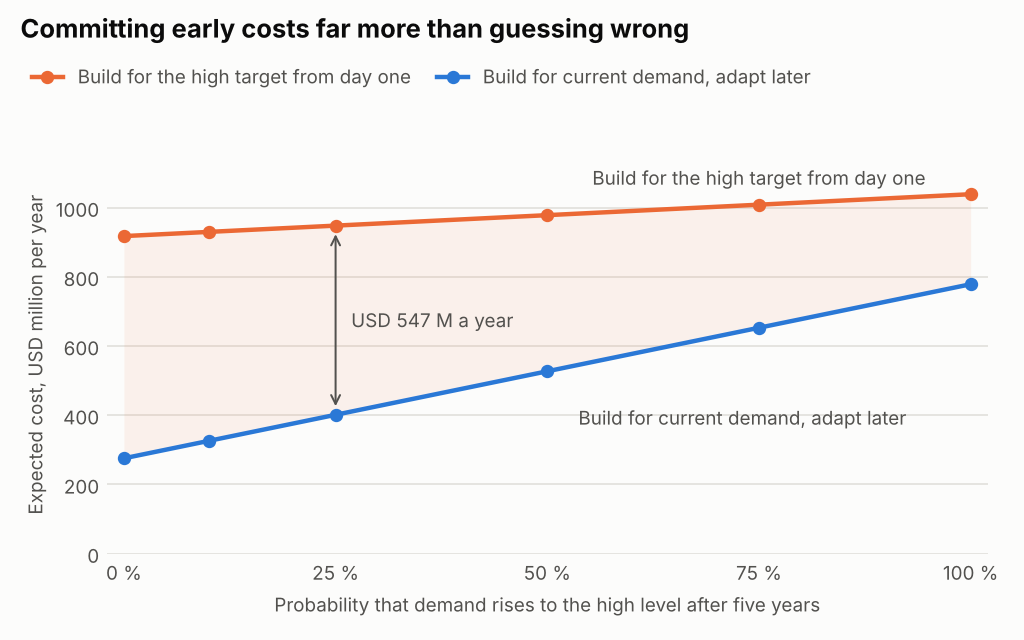
\includegraphics[width=0.72\textwidth]{fig_cost_vs_p.png}
\caption{Expected annual cost of building for the high target and of the adaptive rule.}\label{fig:p}
\end{figure}

Building for the high demand target from the outset costs \musd{} 948 a year at $p=0.25$, against \musd{} 401 for the
adaptive rule: a gap of \musd{} 547 a year, or about USD 32 per person. Even if demand is certain to rise after five
years, early commitment costs a third more, because oversized systems are paid for during the years in which
demand is still low.

\subsection{The value of stochastic planning and of information}
The adaptive rule is within 0.1\,\% of the stochastic optimum at $p=0.25$, 0.5\,\% at $p=0.5$ and 2\,\% at $p=1$.
Perfect information about future demand would lower cost by less than 1\,\%. Once systems can be expanded or
replaced, knowing demand in advance is worth little; what matters is not having committed. At $p=0.25$ the
optimal first-stage plan gives stand-alone solar to 67\,\% of people and small mini-grids to 33\,\%.

\subsection{When does a swarm-grid option matter?}
With the swarm option in its central case, expected cost falls by 1.0\,\% at $p=0.25$ and 1.6\,\% at $p=0.5$, and
19\,\% of people start with a swarm grid (58\,\% stand-alone solar, 23\,\% mini-grid). Table~\ref{tab:swarm} shows
that the result hinges on the generation premium.

\begin{table}[!ht]\centering\small
\caption{Reduction in expected cost from adding the swarm option (\%), by generation premium $\pi$ and fixed cost
$F_{SW}$; line cost USD 2,000 per km.}\label{tab:swarm}
\begin{tabular}{lrrrrrr}\toprule
 & \multicolumn{3}{c}{$p=0.25$} & \multicolumn{3}{c}{$p=0.50$}\\
$\pi$ \textbackslash{} $F_{SW}$ & 0 & 2,500 & 5,000 & 0 & 2,500 & 5,000\\\midrule
0 & 9.4 & 7.8 & 6.5 & 11.2 & 9.3 & 7.8\\
0.15 & 4.5 & 3.3 & 2.3 & 5.9 & 4.4 & 3.1\\
0.30 & 1.9 & 1.0 & 0.4 & 2.9 & 1.6 & 0.7\\
0.50 & 0.3 & 0.0 & 0.0 & 0.6 & 0.1 & 0.0\\
0.75 & 0.0 & 0.0 & 0.0 & 0.0 & 0.0 & 0.0\\\bottomrule
\end{tabular}
\end{table}
A swarm grid that generates as cheaply as a mini-grid would cut expected cost by 8 to 11\,\%. With a premium of
50\,\% or more the option is never chosen. The fixed cost matters less than the premium.

\subsection{Compatibility}
\begin{table}[!ht]\centering\small
\caption{Expected cost under alternative compatibility assumptions (\musd{} per year, stochastic optimum).}\label{tab:compat}
\begin{tabular}{lrr}\toprule
 & $p=0.25$ & $p=0.50$\\\midrule
Without swarm option, stand-alone systems stranded by a mini-grid (baseline) & 400.7 & 524.4\\
Without swarm option, stand-alone systems reusable in a mini-grid & 391.4 & 507.3\\
With swarm option, central case ($\chi_{SA,SW}=\chi_{SW,MG}=1$, $\chi_{SA,MG}=0$) & 396.8 & 516.2\\
With swarm option, swarm hardware stranded by a mini-grid & 398.5 & 520.2\\
With swarm option, stand-alone systems not reusable in a swarm & 398.7 & 519.9\\
With swarm option, stand-alone systems reusable in a mini-grid & 390.2 & 505.6\\\bottomrule
\end{tabular}
\end{table}
Making stand-alone systems reusable when a mini-grid arrives lowers expected cost by 2.3 to 3.3\,\%, more than the
swarm option does in its central case. About half of the swarm option's value is lost if its hardware is stranded
by a later mini-grid. The two are substitutes: once stand-alone systems can be absorbed into a mini-grid, adding the
swarm option lowers cost by only 0.3\,\%. In this model the swarm grid earns its place mainly as a bridge between
technologies that would otherwise not be compatible.

\subsection{Robustness}
Across first-stage lengths of 3 to 8 years, discount rates of 5 to 12\,\% and capital shares of 0.60--0.70 to
0.90--0.95, the cost ratio of building for the high target to the adaptive rule ranges from 2.1 to 2.7 at
$p=0.25$ and from 1.6 to 2.2 at $p=0.5$; the adaptive rule stays within 0.9\,\% of the stochastic optimum; and the
swarm option's value stays between 0.7 and 1.8\,\% (\texttt{national/results/robustness.csv}).

\section{Village-level evidence}
Two companion analyses in the repository look inside the settlement. A multi-stage network-design model of one
village (\texttt{swarmplan/}) finds that interconnecting nanogrids pays only when poorer nanogrids cannot finance
their own equipment, that a central hub feeding a swarm beats a classic mini-grid, and that the value of a staged
upgrade disappears when swarm hardware is stranded by the hub. Applying the decision framework of
\citet{ouanes2026} to 2,075 settlements around Antongil Bay and Ambanja (\texttt{case\_study/}) shows that the
framework approves or defers all settlements alike, depending on whether budget limits are assumed, and that once
line costs are added the verdict turns on the demand level. Both point the same way as the national result: the
case for the middle option rests on modularity and compatibility, not on cost savings from sharing energy.

\section{Discussion}
The results suggest three practical points. First, demand targets in geospatial plans should be read as
destinations, not as sizing instructions: the cost of sizing for a destination that is years away exceeds the cost
of any forecast error. Second, plans would gain more from recording which investments keep options open than from
more elaborate optimisation; a myopic rule with re-planning is near-optimal here. Third, technical standards that
let small solar systems be absorbed into later networks have a measurable value at national scale, and they are the
condition under which swarm grids are worth more than a cheaper mini-grid.

\section{Limitations and next steps}\label{sec:limits}
\begin{itemize}
\item \textbf{Inputs.} The settlement data are the platform's 2019 inputs. No official specification file was
available; household sizes, grid cost and tiers follow the published scenario description, while grid losses,
grid investment cost and the intermediate access target are assumed.
\item \textbf{Two demand levels, one probability.} Demand is either Tier~1 or Tier~3, with a common probability.
A distribution of demand paths, and probabilities that vary with remoteness or market access, are the next step.
\item \textbf{Service quality.} Stand-alone solar at Tier~3 is treated as equivalent to a mini-grid connection.
\item \textbf{Switching costs.} Stranding is a share of levelised cost; capital shares are assumed. Running costs of
oversized systems are approximated.
\item \textbf{Swarm costs.} The premium, fixed cost and line cost are not based on field data. Operators of mesh
and nanogrid systems could supply them; \citet{crossboundary2025} report a 41\,\% lower capital cost per connection
for a full mesh-grid site than for a conventional mini-grid in Nigeria, and a higher cost where mesh-grids extend an
existing network.
\item \textbf{Adaptation.} Expansion and replacement are immediate and cost nothing beyond stranded capital. There
are no construction lags, transaction costs or lost consumption during an upgrade; all of these would favour
building somewhat ahead of demand.
\item \textbf{Grid.} Settlements reached by the grid in either plan are excluded. Later grid arrival, and
arrangements in which mini-grids operate under the grid \citep{gonzalezgrandon2021}, are not modelled.
\item \textbf{Behaviour.} Operators are cost-minimising. Market power and tariff regulation
\citep{bougebrael2026} are left to the village model.
\end{itemize}

\section{Conclusion}
For a third of Madagascar's population the least-cost electrification technology depends on an assumption about
future demand. Treating that demand as uncertain shows that the main risk is not choosing the wrong technology but
sizing for a future that has not arrived. A plan that builds for current demand and adapts is near-optimal; an
intermediate swarm-grid option adds a few percent when its generation is not much dearer than a mini-grid's and
when hardware can be carried over.

\bibliographystyle{plainnat}
\bibliography{refs}
\end{document}
